\subsection{Blockchain}
% 
Since the inception of a digital currency Bitcoin (described in the following section) in 2009, blockchain has been part of the discussions about Bitcoin's novel approach to currency. Over the time, the perception shifted from seeing blockchain as a part of Bitcoin's system into seeing it as an separate, disruptive technology. Some media even mark \textit{blockchain} to be the word of the year 2017\footnotemark, while others comparable it to inception of the Web in 1990s \cite[p. 14]{Swan2015BlockchainEconomy}.
% 
\footnotetext{https://www.theguardian.com/technology/2018/jan/30/blockchain-buzzword-hype-open-source-ledger-bitcoin, accessed 28-03-2018}

Blockchain is a public ledger, that contains all the transactions of the cryptocurrency to date \cite{Swan2015BlockchainEconomy}. It is distributed among all the computers participating in the consensus process. Since it contains all the past transactions (since the inception of the currency), it is never wiped clean. All changes happen as amendments to the latest version of the blockchain.

A change could be any bunch of data. For example it could be a number of latest transactions (as is the case with Bitcoin) or newly deposited agreements (as in Quorum - enterprise level ledger \footnotemark ). This is called a \textit{block}. Blocks are the fundamental parts, that make up the blockchain. When a new blockchain is created, a first set of changes becomes the first block.
% 
\footnotetext{Quorum is a blockchain-based private storage for agreements. Its intended users are enterprises in the finance industry, who are trading financial derivatives and who need to reach an agreement, while maintaining acceptable level of privacy.
\begin{flushleft}
http://fortune.com/2016/10/04/jp-morgan-chase-blockchain-ethereum-quorum/, accessed 28-03-18
https://www.jpmorgan.com/global/Quorum, accessed 28-03-18
\end{flushleft}
}
% 
When more changes need to be made (for example, more transactions need to be processed), a new block is created. The creation of a new block involves computing a hash value of the previous block. This hash value is then included in the new block, together with the data. By including the hash value in the new block, these two are now linked. All the blocks are linked together in such fashion. Figure \ref{fig:blockch-basics} illustrates this principle. 
% 
\begin{figure}[t]
    \centering
    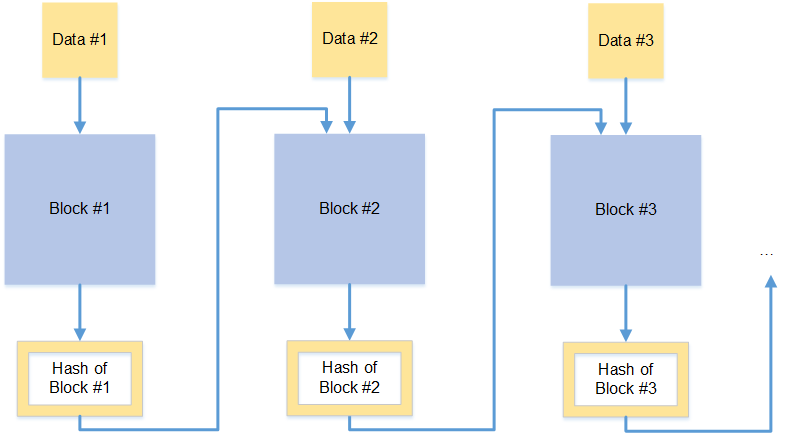
\includegraphics[width=.95\textwidth]{blockchain-basics}
    \caption{The basic architecture of a blockchain. If Block \#1 is the first block in the chain, it is also referred to as the \textit{genesis block}.}
    \label{fig:blockch-basics}
\end{figure}

It is not possible to alter the past blocks in the blockchain. In order to do this, we would need to find such combination of data, that would produce the same hash, which violates the pre-image resistance property of the hash function. Alternative technique could be to change the data in block n, then calculate new hash and include it in block n+1 and so on, recalculating every subsequent block. However, the decentralisation of the blockchain prevents this. Every participating node maintains and updates its own copy of the blockchain. When there is a dispute about what is the correct version of the blockchain, the version that is present on most nodes is chosen as the `correct' one and the other versions are discarded. This means, that an attacker would need to control majority of the nodes in the network in order to include counterfeit data in the blockchain.

Based on the data we include in the blockchain, we can distinguish between three `levels' \cite{Swan2015BlockchainEconomy}. \textit{Level 1} is blockchain used with currency only. The data here are transactions of that currency. Level 1 of blockchain would be for example Bitcoin. \textit{Level 2} includes smart contracts and more advanced transactions and agreements than Level 1. However, Level 2 of blockchain is still tied to financial applications in some way. Example of Level 2 blockchain is Ethereum platform. \textit{Level 3} of blockchain includes usage outside of financial applications, in sectors such as government or health-care \cite{Swan2015BlockchainEconomy}.


% Motivate problems with cryptocurrency? Double spending problem and byzantines general problem? 

% Central bank system - problems?

% Decentralised system - solutions

% mentioned briefly - drawbacks

% narrower definition of blockchain - list of transactions for a cryptocurrency

% broader definition - number of other applications, Blockchain 2.0 and Blockchain 3.0 as described by Swan